\section{Rancangan Solusi}

\begin{figure}[ht]
  \centering
  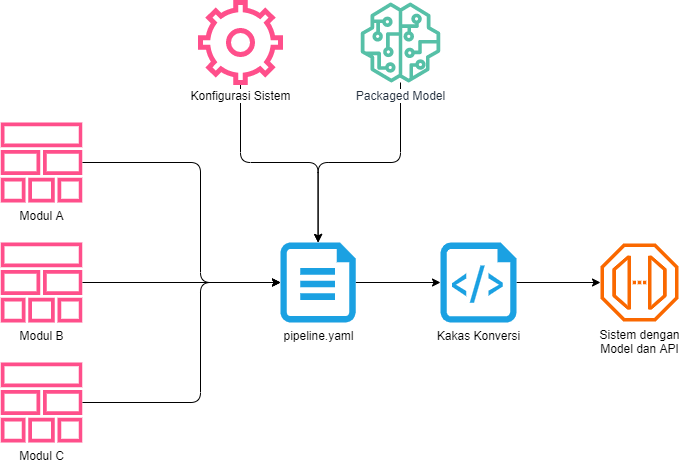
\includegraphics[width=0.7\textwidth]{03-rancangan-solusi.drawio.png}
  \caption{Rancangan Solusi Konversi Eksperimen}
  \label{fig:03-tool}
\end{figure}

Dalam makalah ini, dibuat suatu prototipe kakas yang dapat menganalisis suatu eksperimen dan mengubahnya menjadi suatu sistem yang siap (lihat Gambar \ref{fig:03-tool}).
Definisi dari perjanjian data yang menjadi masukan dan keluaran akan dibuat oleh sistem secara otomatis berdasarkan eksperimen.
Alur pemrosesan yang didefinisikan dapat dibuat lewat \textit{markup file} seperti JSON atau YAML yang formatnya sudah ditentukan untuk kakas tersebut.
Alur didefinisikan lewat pemanggilan modul-modul yang diimplementasikan lebih dulu yang nantinya dapat memanggil sebuah model yang biasanya sudah siap dan disimpan dalam sebuah file.

Modul dapat diimplementasikan dalam bahasa apapun selama semua modul yang digunakan menggunakan bahasa yang sama.
Dalam pendekatan yang umum, digunakan Docker sebagai bantuan untuk melakukan pemrosesan terhadap data, karena hal ini diterapkan dalam sebuah \textit{pipeline} eksperimen.
Dalam sebuah sistem yang berjalan, hal ini menjadi kurang baik karena akan memerlukan komputasi yang lebih berat akibat penggunaan virtualisasi.

Hasil akhir dari kakas ini adalah sebuah kode sistem yang siap digunakan untuk \textit{production}.
Kakas ini tentunya bersifat \textit{non-domain specific} atau dapat digunakan untuk kasus pembuatan sistem inferensi secara umum.
Pemilihan \textit{interface} untuk model ditentukan lewat \textit{markup file} yang telah dibuat.
Metode komunikasi yang akan diimplementasikan adalah REST sebagai contoh dari \textit{interface} yang umum digunakan dalam sistem.

Penulis mengimplementasikan kakas ini dalam bahasa Go.
Hasil dari proses konversi yang dilakukan kakas akan berupa kode program dalam bahasa Python dengan \textit{FastAPI}.

